\section{Menu Design}
\label{designmenu}
\todo{This section describes the design choices made when creating our menu.}
To keep the same look and feel throughout the whole \ac{giraf} project, we looked for inspiration in the projects from 2012. The \ac{wombat} project had the same kind of customisation menu we were looking to make \autoref{fig:wombat}. We followed the same basic design idea as in \ac{wombat}, but with a different customisation part (the part at the very right). The left half of the screen contains a list of children associated with the current guardian and a list of already saved games. The right half is a customisation part where you can add, remove, and edit stations. We chose a list approach for this as well, to keep the whole activity separated in three lists with roughly the same design.

When an application is run from the Launcher, the application receives a color that can be chosen in the Launcher. We use this color to set the overall color theme of the menu, meaning that the whole menu will show in the chosen color from the Launcher.
To ease the process of finding that game that you are looking for, the saved games will have a picture attached to them. This picture represents the category of the first station in that game configuration.

\subsection{Flow}
To show the functionalities of the menu, the natural flow will be shown in this section.
\begin{figure}[H]
\centering
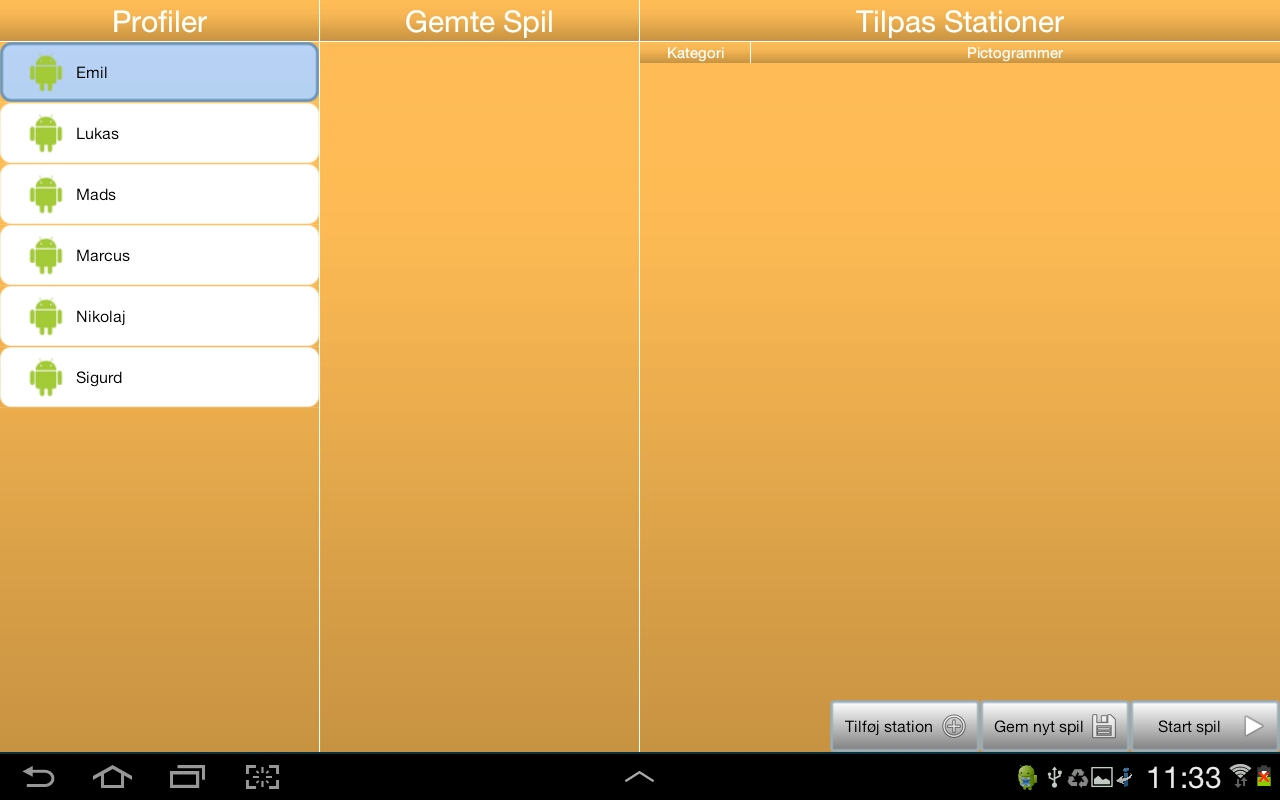
\includegraphics[width=1.0\linewidth]{img/screenshots/profile_flow_1.jpg}%0.1 margin
\caption{The main activity.}
\label{fig:profile_flow_1}
\end{figure}
\autoref{fig:profile_flow_1} shows the general design of the menu. The overall color theme (Orange in this example) can be changed from the Launcher. The menu is divided into three parts; profiles, saved games, and game customisation. When the application is launched the menu will appear and the profile list will be populated with the children associated to the current guardian. In this example "Emil" has been chosen, but there are no saved games related to that child, yet.
We will now continue to push the "Tilføj station" (Add station) button three times.

\begin{figure}[H]
\centering
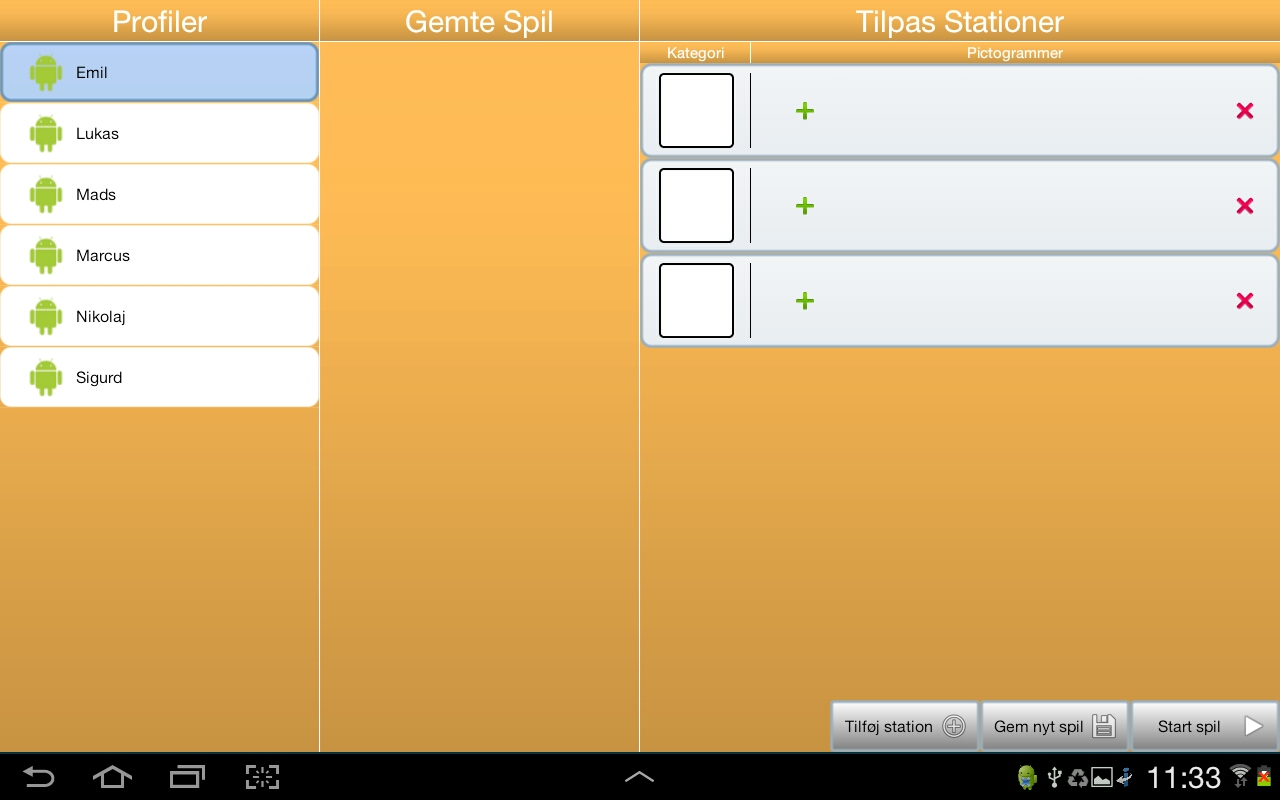
\includegraphics[width=1.0\linewidth]{img/screenshots/profile_flow_2.jpg}%0.1 margin
\caption{The main activity with three stations.}
\label{fig:profile_flow_2}
\end{figure}

The game customisation part of the menu has now been populated with three elements, each representing a station. An element/station consists of three buttons:
\begin{itemize}
\item \textbf{Add category:} Pressing the category pictogram will allow you to choose a different one. It is blank on default to show that no category has been selected.
\item \textbf{Add pictograms:} Pressing the green "+" will allow you to select the pictograms you want to be associated to the category.
\item \textbf{Delete station:} Pressing the red "x" will delete the station.
\end{itemize}
We will now continue to select a category for the first station by pressing the add category button.

\begin{figure}[H]
\centering
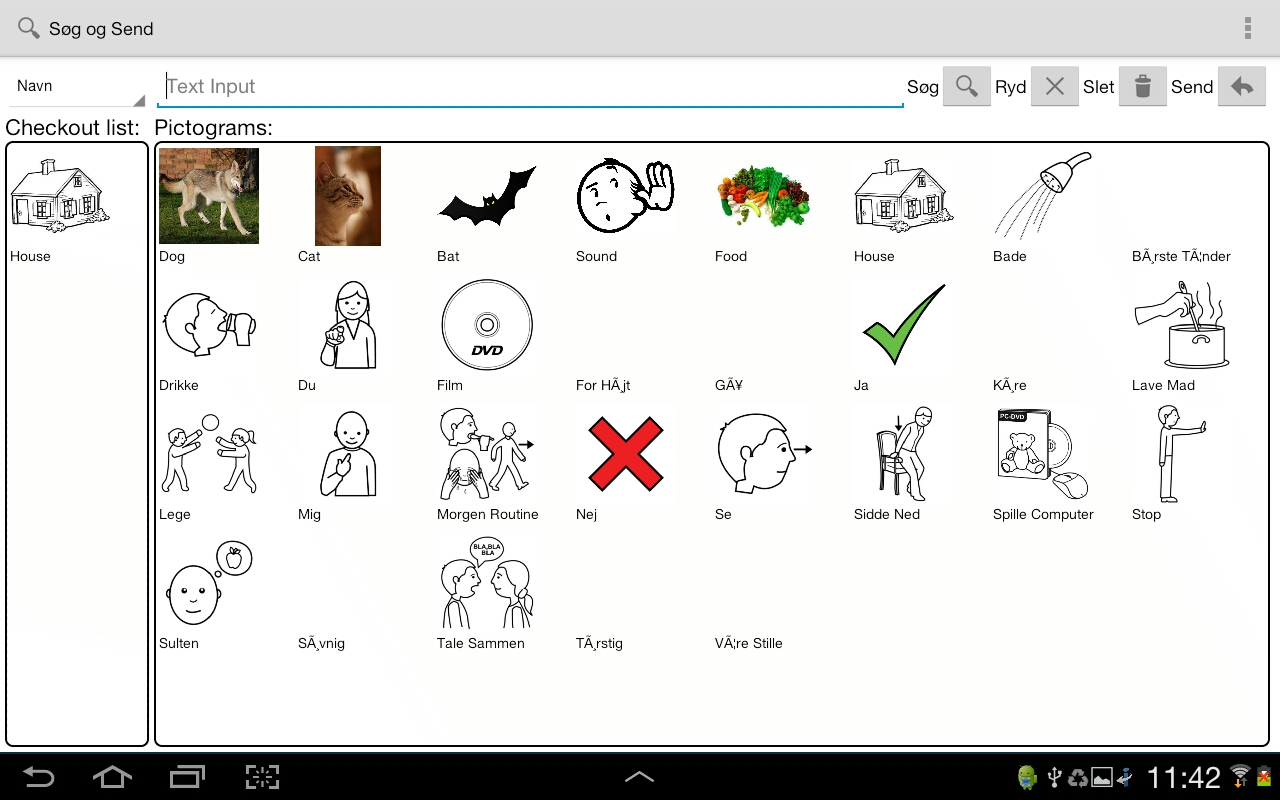
\includegraphics[width=1.0\linewidth]{img/screenshots/profile_flow_3.jpg}%0.1 margin
\caption{\ac{cat} with one pictogram selected.}
\label{fig:profile_flow_3}
\end{figure}

\autoref{fig:profile_flow_3} shows that \ac{cat} opens to allow you to select a pictogram to use for the category.
The pictogram "House" has been selected in this example, and we will now continue to press the "Send" button. This will send the pictogram back to the menu.

\begin{figure}[H]
\centering
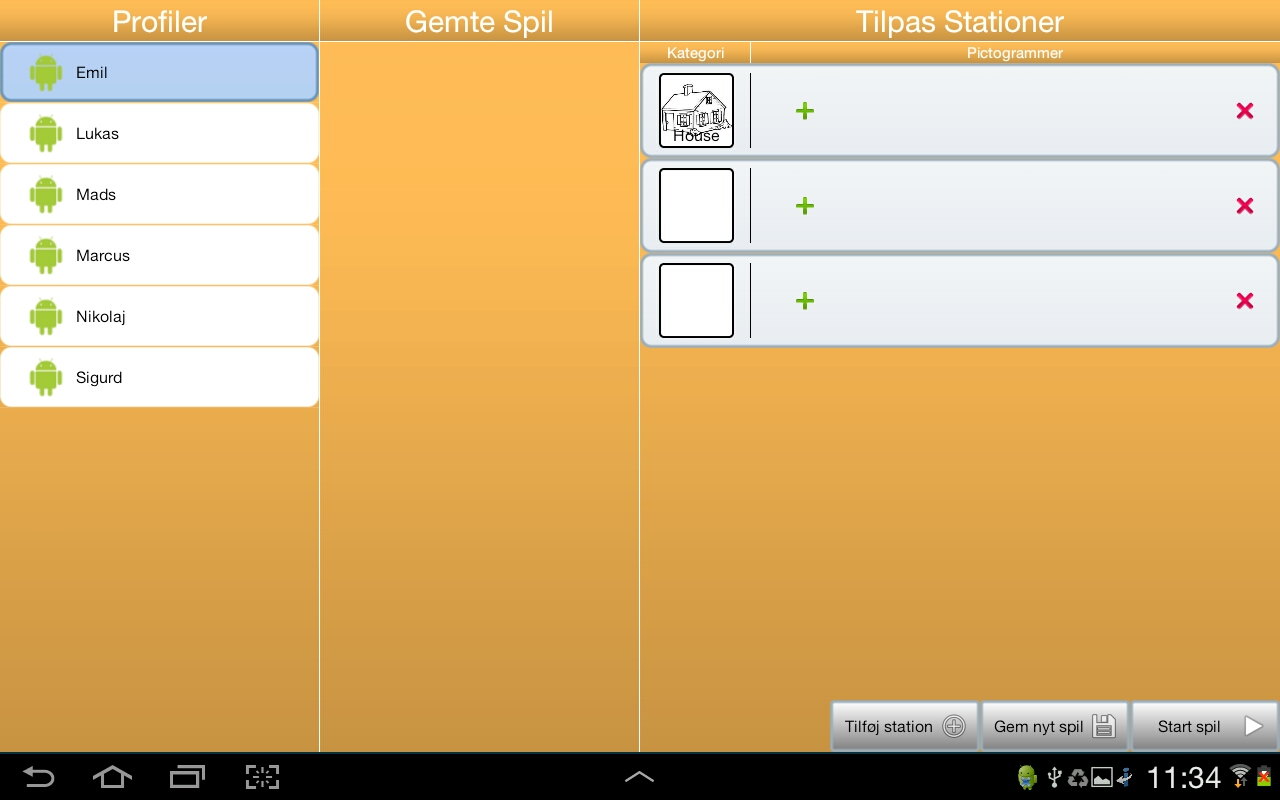
\includegraphics[width=1.0\linewidth]{img/screenshots/profile_flow_4.jpg}%0.1 margin
\caption{The main activity with one category chosen.}
\label{fig:profile_flow_4}
\end{figure}

It can now be seen in \autoref{fig:profile_flow_4} that the pictogram we selected before has been set as the category for the first station. We will now press the green "+" to add the pictograms we want associated with this category.

\begin{figure}[H]
\centering
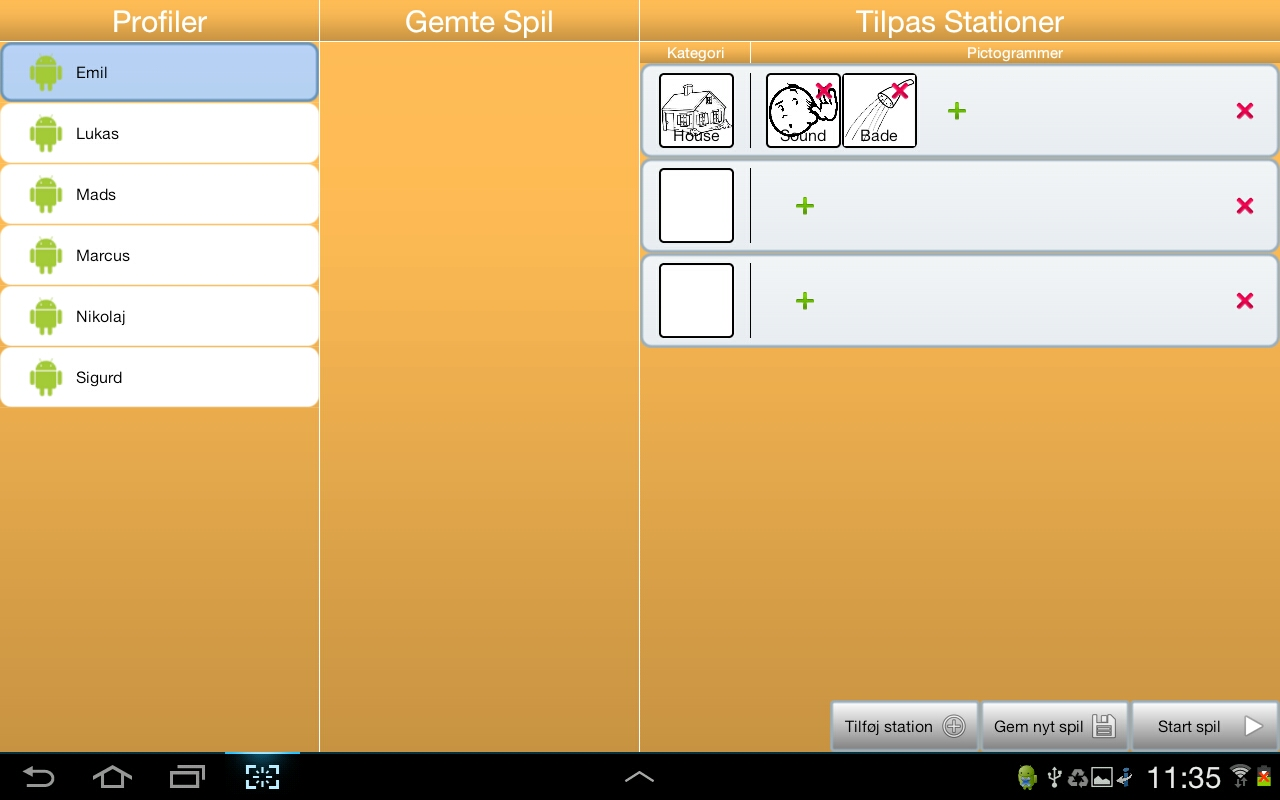
\includegraphics[width=1.0\linewidth]{img/screenshots/profile_flow_5.jpg}%0.1 margin
\caption{The main activity with one complete station.}
\label{fig:profile_flow_5}
\end{figure}

It can be seen in \autoref{fig:profile_flow_5} that two pictograms was selected, again via PictoSearch. \todo{Acronym for PictoSearch, go!} We will proceed to add categories and pictograms to the remaining stations, using the same method.

\begin{figure}[H]
\centering
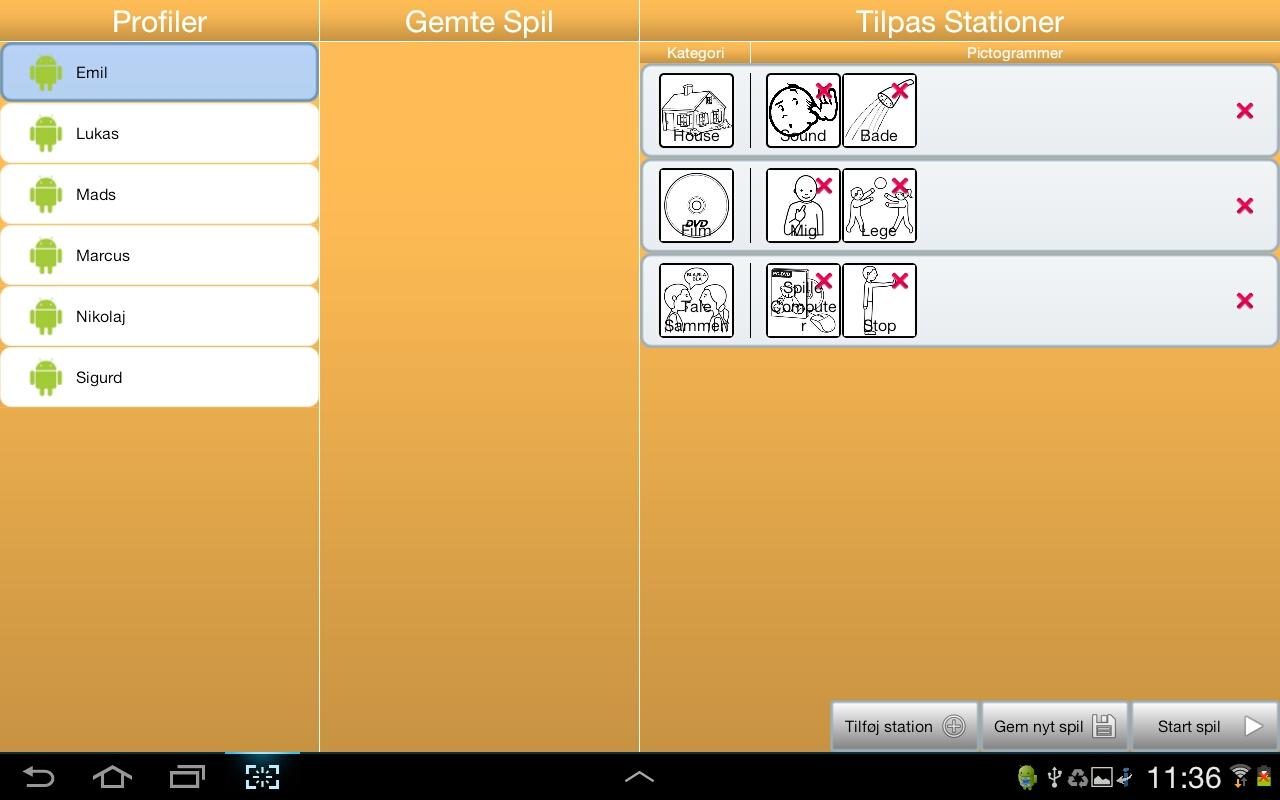
\includegraphics[width=1.0\linewidth]{img/screenshots/profile_flow_6.jpg}%0.1 margin
\caption{The main activity with three complete station.}
\label{fig:profile_flow_6}
\end{figure}

\autoref{fig:profile_flow_6} shows that the three stations have now been filled with pictograms. Note that the green "+" is gone, this is because we only allow a total of six pictograms. We will now press the "Gem nyt spil" button to save the game.

\begin{figure}[H]
\centering
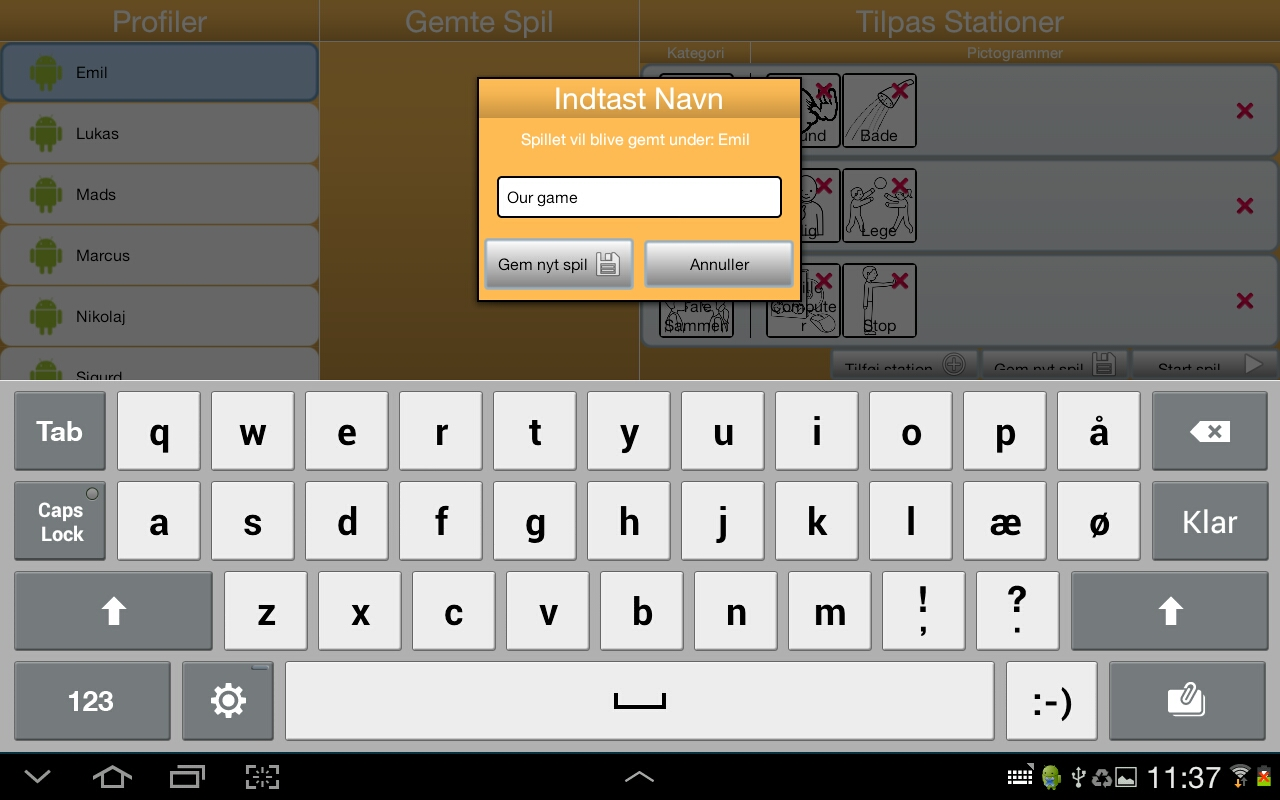
\includegraphics[width=1.0\linewidth]{img/screenshots/profile_flow_7.jpg}%0.1 margin
\caption{Save dialog.}
\label{fig:profile_flow_7}
\end{figure}

\autoref{fig:profile_flow_7} shows that a dialog appears when the save game button has been pressed. This dialog allows you to enter a name for your game and save it. We will call our game "Our game" and press "Gem nyt spil" which will save the game.

\begin{figure}[H]
\centering
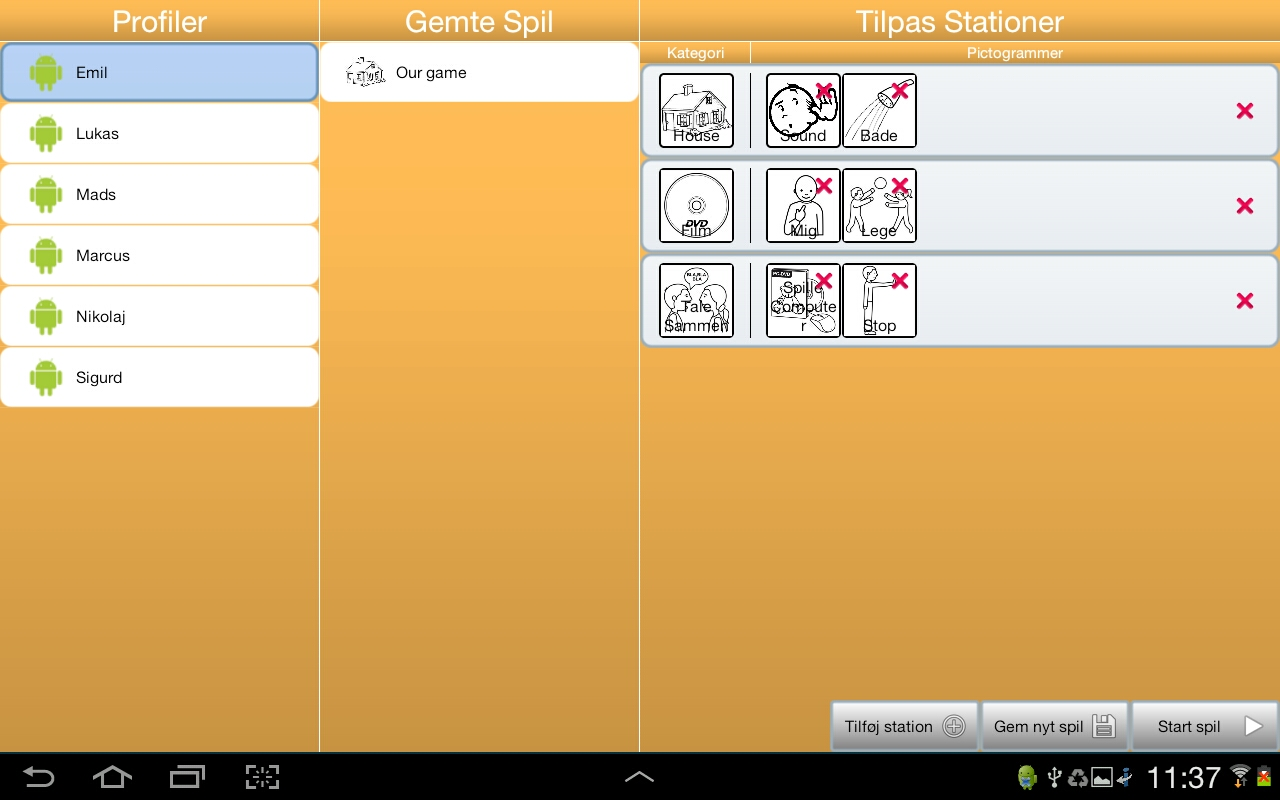
\includegraphics[width=1.0\linewidth]{img/screenshots/profile_flow_8.jpg}%0.1 margin
\caption{Complete example of the main activity.}
\label{fig:profile_flow_8}
\end{figure}

The game configuration has now been saved, and is shown in the list of saved games. See \autoref{fig:profile_flow_8}.\\
The newly saved game is linked to "Emil", and will be shown whenever he is selected.\\\\
To delete a saved game you will simply have to do a long click on the game you wish to delete. This will prompt you to whether you are sure or not. If deleted, the game will disappear from the list and the configuration will be deleted from the database.
